\FloatBarrier
\subsection{Characterizing sources of fine-scale auroral structure}\label{sec:aurorabasic}
The optically thin aurora with observed optical intensity $\mathscr{I}$ due to auroral volume emission rate (VER) $p$ looking along direction $\vect{r}$ is described by
\begin{equation}\label{eq:bint}
\mathscr{I} = \int_0^\infty p(\vect{r})\textrm{d}\vect{r}
\end{equation}
implying that ground-observed auroral brightness strongly depends upon viewing angle.
Additional important factors such as wavelength-dependent atmospheric absorption between the aurora and observer are detailed in chapter~\ref{chapter:sim}.
Non-uniqueness of the observational system is implicit in (\ref{eq:bint}) as demonstrated with the examples in Figure~\ref{fig:bint} for an optically thin 2-D phantom. 
\begin{figure}\centering
    \begin{subfigure}[t]{0.45\linewidth}\centering
        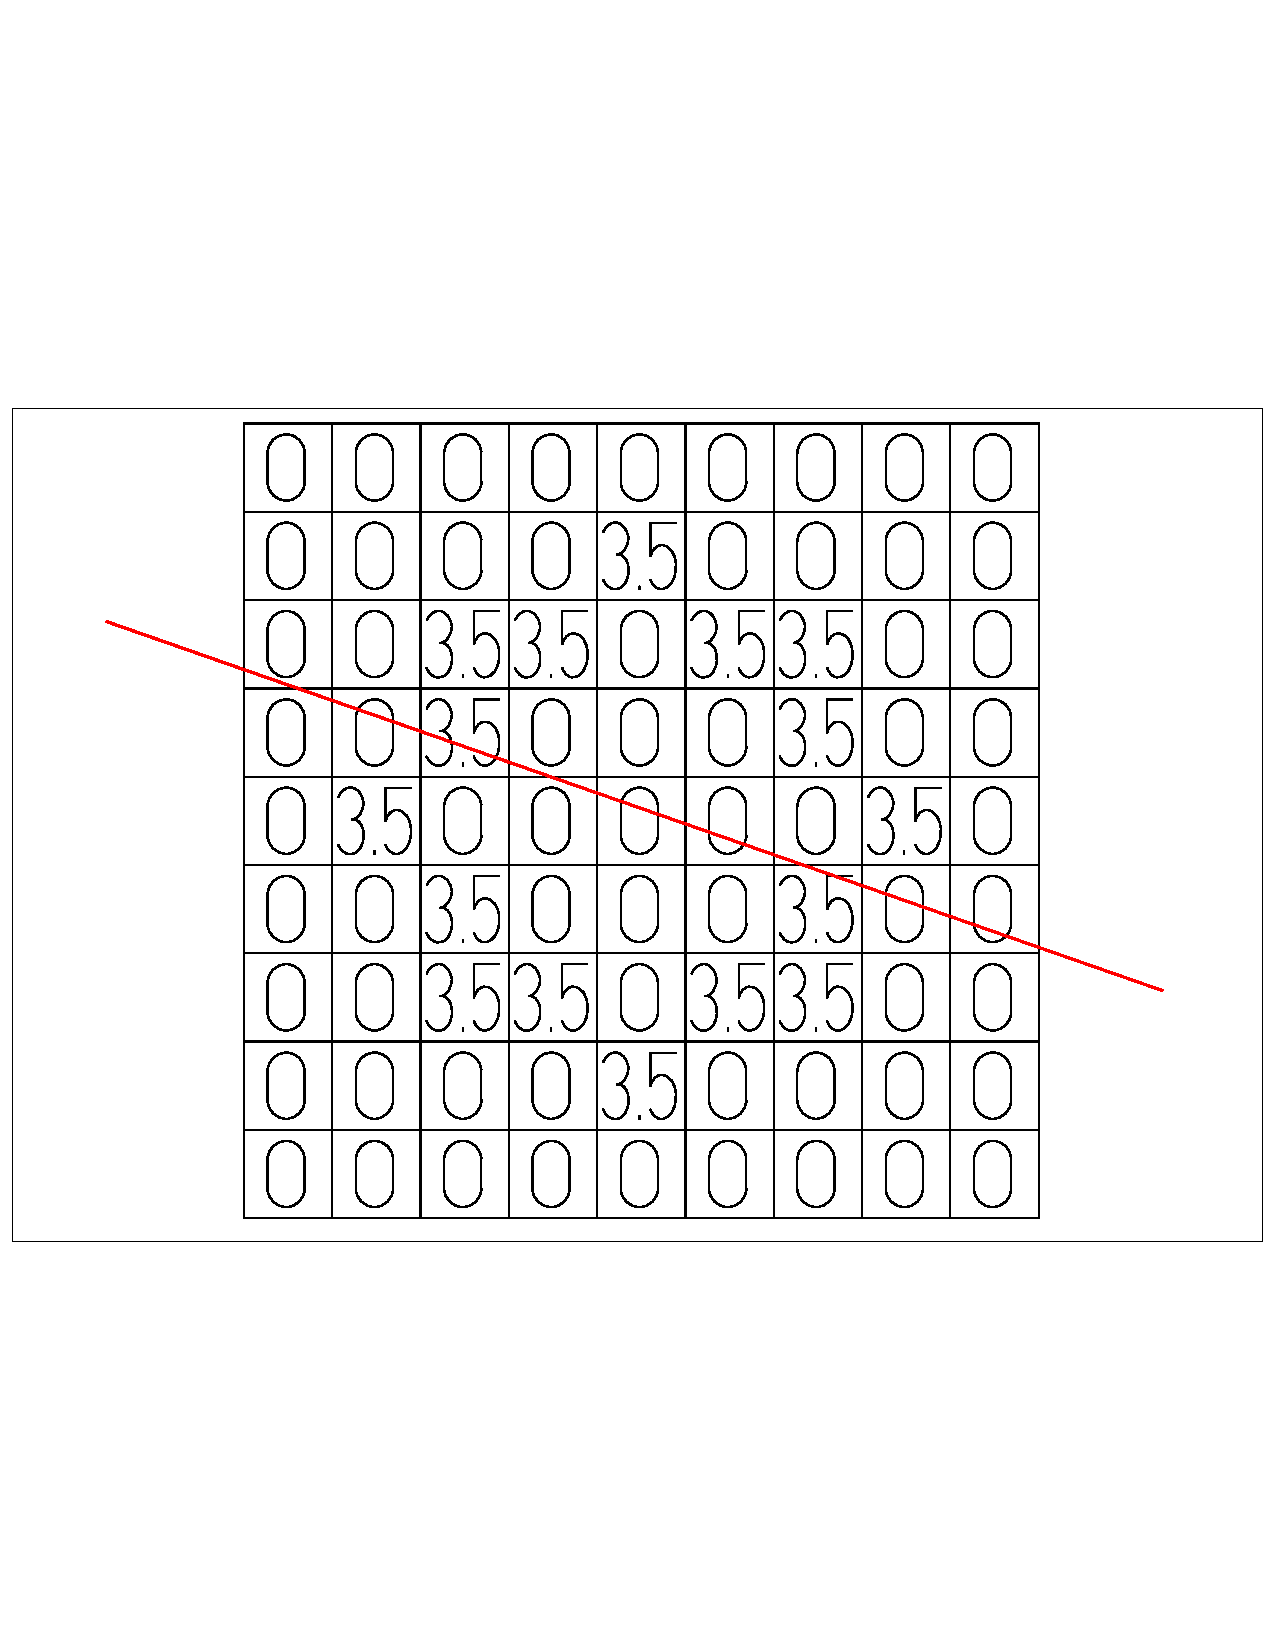
\includegraphics[width=\linewidth,trim=50 200 50 200,clip]{gfx/circle}
        \caption{Hollow optically thin structure with line-of-sight.}		
    \end{subfigure}
    \begin{subfigure}[t]{0.45\linewidth}\centering
        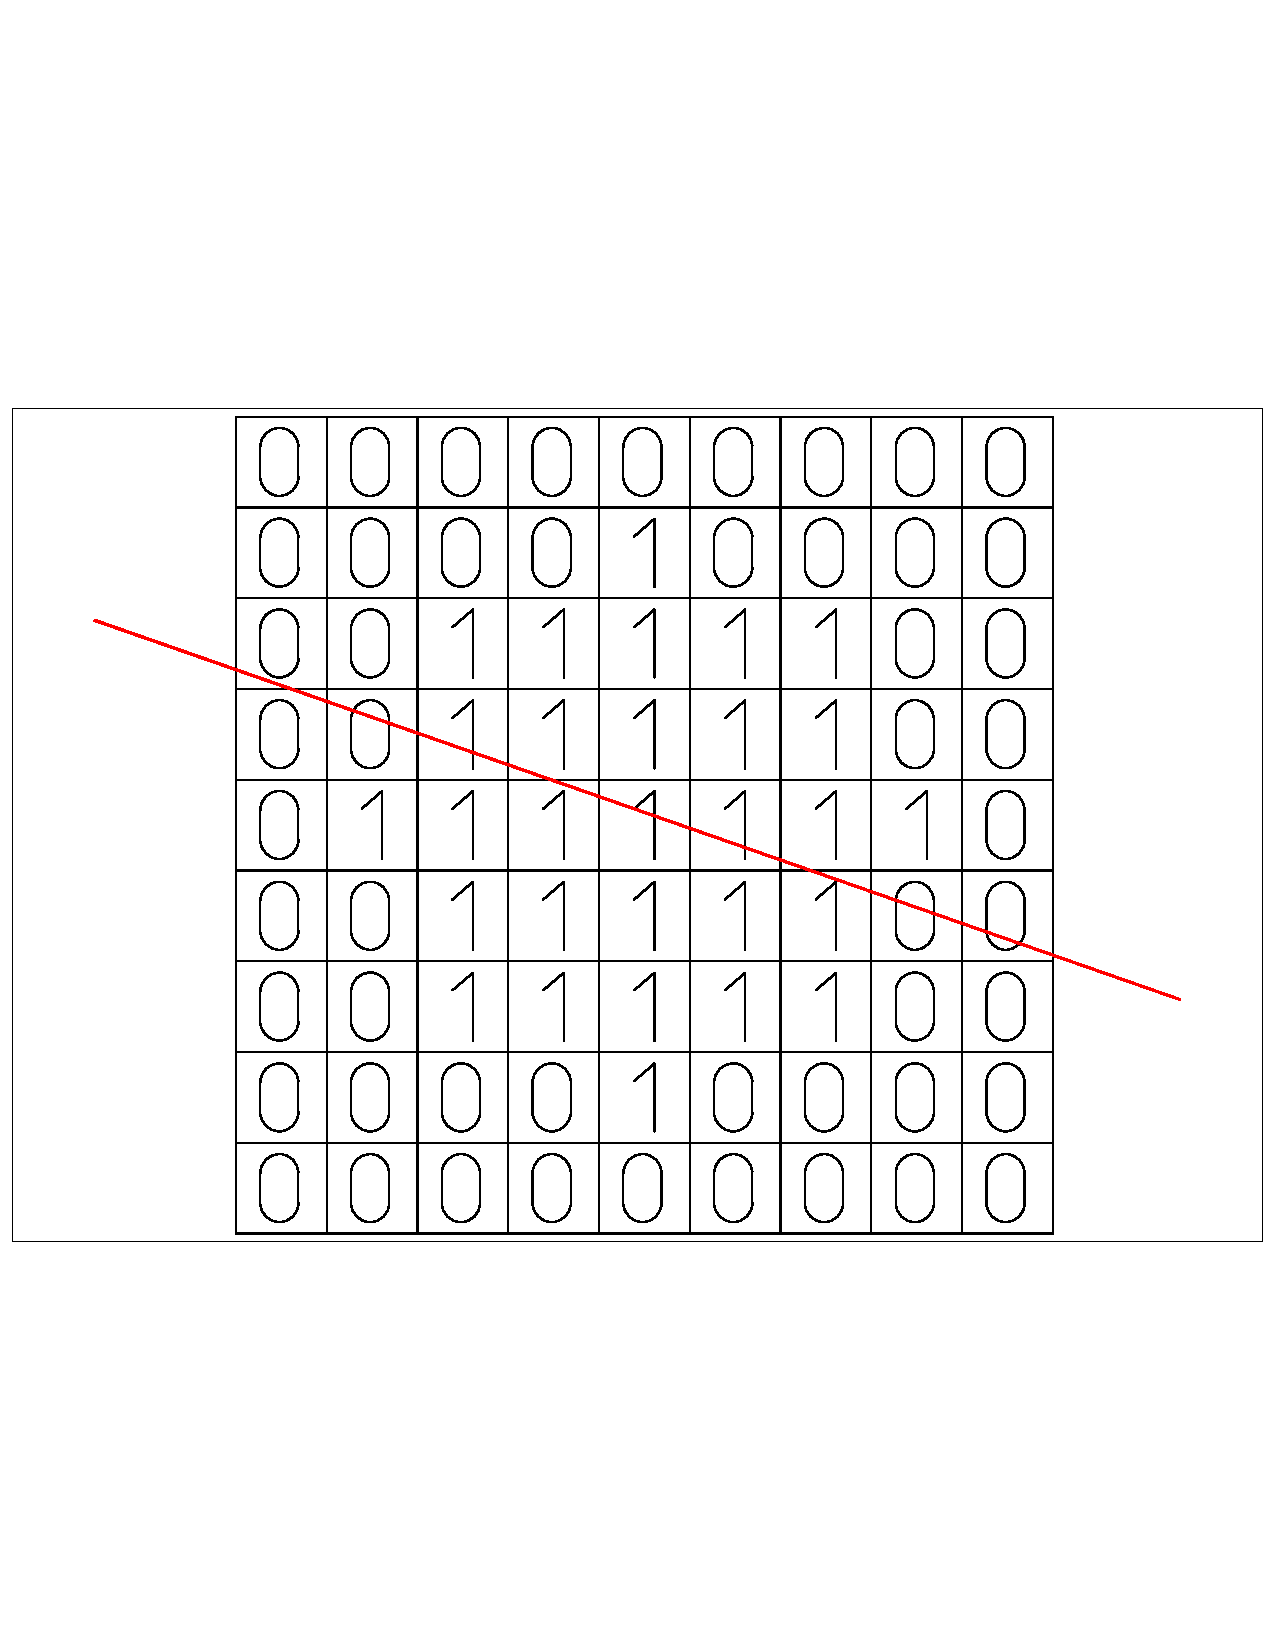
\includegraphics[width=\linewidth,trim=50 200 50 200,clip]{gfx/disk}
        \caption{Filled optically thin structure with line-of-sight.}		
    \end{subfigure}
    \caption{Optically thin phantoms with red line-of-sight integral. Completely distinct forms after line-integration give the same result, an example of the non-uniqueness problems inherent to auroral remote sensing.}\label{fig:bint}
\end{figure}
Whether the observed target is disk, circle, spline or other arbitrary form, line integration of distinct forms can lead to the same integrated (observed) result.

We assume the auroral cameras are boresight-aimed at magnetic zenith. 
Non-uniqueness becomes increasingly important for large camera viewing angle from magnetic zenith $\theta \gg \unit[1]{degree}$.
As camera ground spacing increases beyond $x \sim \unit[10]{km}$ increasingly poor resolution of fine detail along $B_\perp$ results as demonstrated in Figure~\ref{fig:camres}.
\begin{figure}
	\begin{subfigure}[t]{0.45\linewidth}\centering
		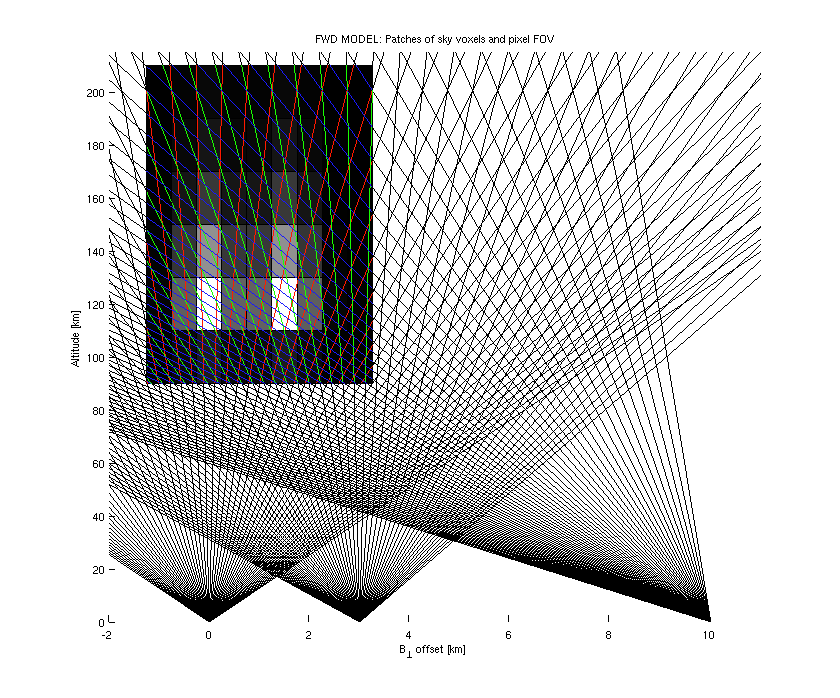
\includegraphics[width=\columnwidth]{../gfx/L3cam}
		\caption{Viewing geometry for auroral arc with cameras at $x \in (0,3,10)$~km.}
	\end{subfigure}
	\begin{subfigure}[t]{0.45\linewidth}\centering
		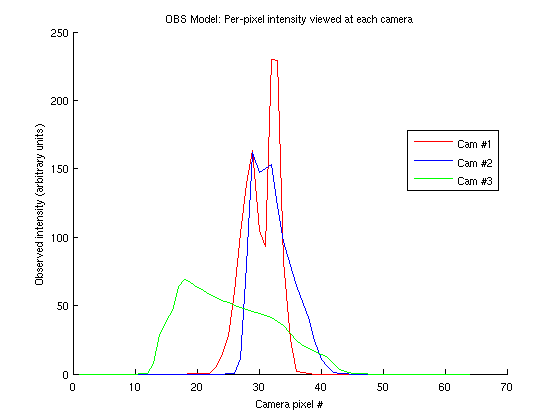
\includegraphics[width=\columnwidth]{../gfx/I3cam}
		\caption{Intensity $I$ for three cameras.}
	\end{subfigure}
	\caption{Notice how the intensity of the green line for $x=\unit[10]{km}$ has smeared out the \unit[1.5]{km} spaced arcs, demonstrating a non-uniqueness issue.}
	\label{fig:camres}
\end{figure}
Figure~\ref{fig:camres}(b) shows the non-uniqueness issue in auroral tomography, particularly for cameras widely spaced from the auroral arc of interest.
Alfvénic splitting auroral arcs with widths in the \unit[0.01..1]{km} range are best observed with cameras spacing $x < \unit[10]{km}$.

The diverse colors and shapes of the aurora have been the focus of human study and speculation for centuries.
The colors of the aurora consist of isolated spectral lines, close groups of spectral lines and continua of spectral bands.
Auroral optical emissions are photons released as excited particles (atoms and molecules, ions and neutrals) relax and emit a photon with wavelengths determined by quantum physics.
The precipitating electron energy at the top of the ionosphere likewise varies between monoenergetic, a band-limited uniform spectrum or a complex spectrum having one or more peaks in a broadband differential number flux spectrum.
% NOTE: example figure here?
Precipitating particle sources include electrons mirroring in the upper ionosphere, particles ejected from the plasma sheet or launched from the magnetotail.
More important to this work than where the electron came from is what acceleration process the particle experienced before crashing into the ionosphere.
Alfvén wave accelerated particles have key signatures in the differential number flux spectrum.
Alfvén wave accelerated electrons kinetically reacting with E- and F-region ionospheric particles give particular signatures in high-speed auroral and ISR observations that are connected observationally in this dissertation.
These factors imply that an appropriate inversion algorithm may yield new science conclusions about the association and characteristics of Alfvénic aurora and plasma turbulence.

Essential to the analyses in this dissertation is the fact that auroral behavior in the $B_\parallel$ dimension may be modeled by numerical solutions to partial differential equations describing energy deposition along a flux tube.
The important \textit{a priori} inputs to such models include solar zenith angle (SZA) (that is, angle of the sun from local zenith).
SZA is commonly used in auroral studies because of the inherent angular ambiguity near the horizon due to refraction. 
When the sun is seen to be at the horizon, the sun is already geometrically below the horizon under typical conditions.
During the day, photodissociation due to solar EUV gives rise to the D-layer ionosphere, absorbing MF.
During solar energetic particle events lower HF wavelengths are also absorbed.

Neutral atoms and molecules along with ions are a prerequisite for structured aurora.
These ionospheric particles are impacted by electrons in finely structured (in $B_\perp$) beams to create structured aurora.
Just before Sputnik I was launched, \citet{chamberlain1957} raised the possibility that locally-accelerated electrons were responsible for fine auroral structure in the E-region, while prior work such as \citet{seaton1954} suggested electrons could not generate E-region aurora.
The first group of Sputnik and Explorer spacecraft in 1957--1958 made structured proton aurora in the E-region seem unlikely and a local acceleration mechanisms for electrons probable \citep{krassovsky1959,wallace1959}.
The primary role of the electron in structured E-region aurora was solidly established by 1960 with \textit{in situ} sounding rocket sensors of increasing fidelity revealing typical scales and dynamics of auroral precipitation.
Of note are the pair of \unit[120]{km} apogee sounding rockets \citep{mcilwain1960} determining the important result that proton particle flux was $\ll 1\%$ electron particle flux, electron energy flux was at least 10 times that of proton energy flux, and small amounts of differential number flux were found.
1963 satellite measurements \citep{sharp1965} at $\unit[8]{ms} \Leftrightarrow \unit[63]{m}$ sampling cadence showed rapidly changing energy spectrum amidst a more slowly changing energy flux.
These observations confirmed that most of the auroral flux had particles less than \unit[10]{keV} with the largest differential number flux at energies $\ll \unit[1]{keV}$.

\subsubsection{Objectives related to characterizing sources of fine-scale auroral structure}
\citet{chaston2007how} noted the characteristics of Alfvénic aurora consistent with the design of the HiST system \citep{hirsch2016}.
The following HiST performance metrics were vital to success:
\begin{enumerate}
	\item Observe aurora with cadence $\leq\unit[20]{ms}$
	\item Operate unattended to catch few seconds of good data from weeks of observation
	\item Time sync between sites $\ll \unit[1]{ms}$ and absolute time sync $\ll\unit[1]{ms}$ for data fusion with other instruments
	\item Physics-based forward model to allow capture of broadband filtered light, enabling fast imaging with comprehensive representation of auroral kinetic reactions in the data inversion process
\end{enumerate}
These metrics were met and exceeded in performance as developed throughout the dissertation.